\section{Compression paddles FE models}
\section{Compresure quality metrics}\label{section:compressionqualitymetrics}
\subsection{Patient comfort}
With a rigid paddle, the breast under compression presents a nearly uniform thickness all over the contact surface. Contrariwise, with a flex paddle, the compressed breast thickness decreases quasi linearly from the chest wall to the nipple. Flex paddles are used to better conform the breast contours and thereby to improve compression. However, Broeders and collegues11 have shown that such compression paddle may decrease the diagnostic quality of mammograms as the breast tissues may be pushed out to the chest wall resulting in less retro-glandular tissue visible on the image. 

\subsection{Image quality }\label{section:averagegalndulardose}
To assess the impact of breast compression on image quality, we inserted a set of microcalcifications into each compressed breast volume. The smallest breast volume contains 21 microcalcifications arranged in a matrix of 7 rows and 3 columns (Figure 4a). The largest breast volume contains 56 microcalcifications arranged in a matrix of 7 rows and 8 columns. The matrix of calcifications is parallel with the entrance surface of the image receptor and positioned at the breast mid thickness (Figure 4b). The distance between two consecutive columns or rows is 10mm. We assumed a uniform breast-equivalent material composed of glandular/adipose tissue with a 20/80 ratio. A mammogram was simulated using typical clinical acquisition parameters obtained with the standard automatic optimization of parameters (AOP) mode. Two simulations were performed with microcalcifications of 0.2 mm and 0.3mm in diameter. The signal-difference-tonoise ratio (SDNR) per pixel of these microcalcifications was measured. Additionally, the signal-to-noise ratio (SNR) was computed on the same pixels excluding the microcalcifications.  


\begin{figure}[!h]
\centering
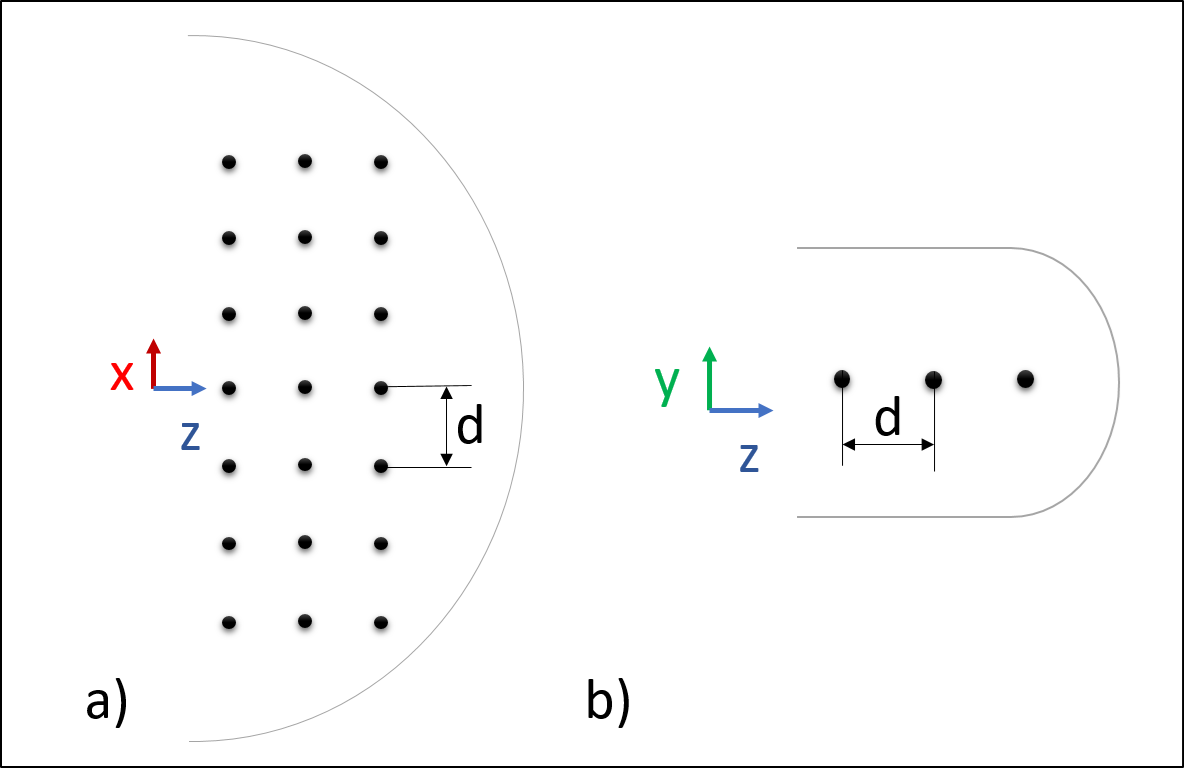
\includegraphics[width=0.5\textwidth,keepaspectratio]{figures/microcalcifications.png} 
\caption{Microclcification distribution over the smallest breast volume $(d=10mm)$: a)axial view, b) sagittal view.}\label{fig:compressionpaddles}
\end{figure}

\subsection{ Average glandular dose}
The average glandular dose (AGD) was derived using the approach proposed by Dance et al12 regardless the paddle type.  In practice, it is very difficult to accurately measure the exact breast thickness. Thus, the nominal breast thickness was used to compute conversions factors which relate measurements of incident air kerma to the delivered mean glandular dose.

\section{Results}\label{section:breastcompressionevaluation}
The force versus breast thickness curves are plotted in Figure 5 for both volunteers with the rigid and flex paddles. We observed a nominal compression thickness roughly equals for both paddles. The resulting internal stress and strain distributions, as well as contact pressure maps were derived at compressive forces of 22 N for the first volunteer (Figure 6) and 95 N for the second one (Figure 7).

\begin{figure}[!h]
\centering
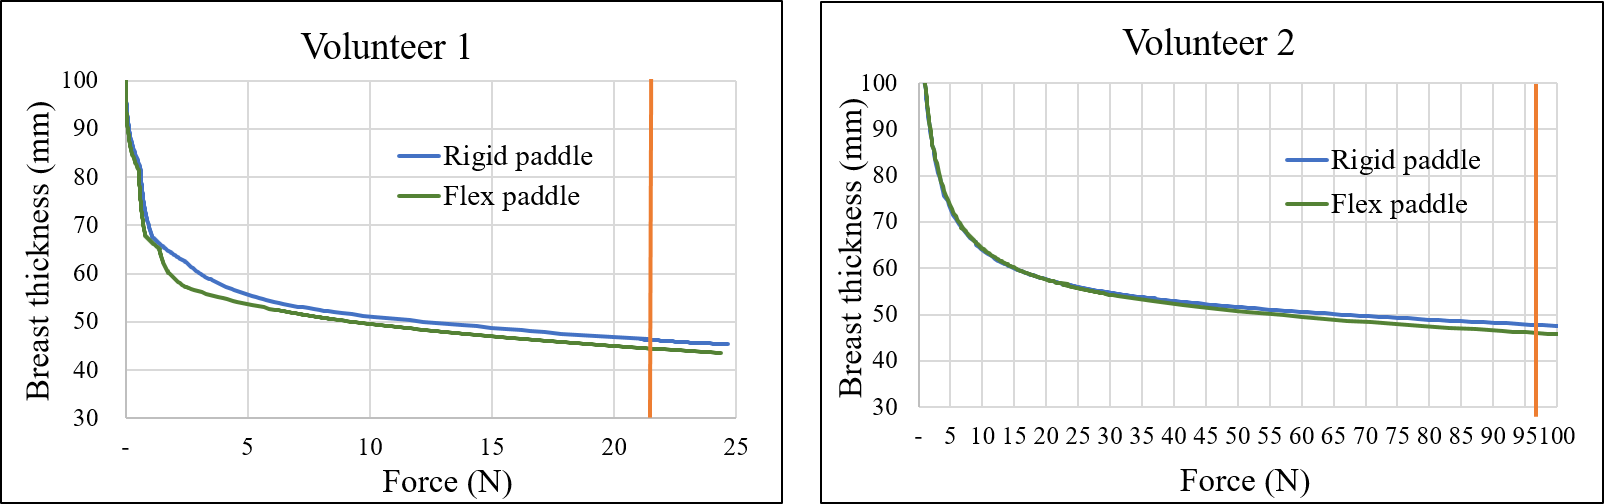
\includegraphics[width=0.9\textwidth,keepaspectratio]{figures/forceThicknessResults.png} 
\caption{Resulting breast thickness for a given compression force}\label{fig:forceThicknessResults}
\end{figure}

As concerns the small breast volume (Figure 6), there is no significant difference between FCP and RCP in pressure distribution over the skin surface or in internal stress/strain intensity distributions. For both compression paddles, high pressure at the skin surface is concentrated in the juxtathoracic region with a maximum pressure of 77.7 kPa. Several clinical studies11,13 sustained this result of no significant difference in experienced pain when using FCP or RCP. In addition, the FE simulations confirm that in small breasts the paddle tilt is too small to impact the tissues compression in the middle part of the breast. 
FCP applied on large breast volumes (Figure 7) results in significantly lower intensities of pressure at the skin surface in contact with the compression paddle, with a maximal pressure of 37 kPa, compared to 56 kPa when using RCP. No significant difference in the measured maximal intensities of strain and stress was observed, however strain and stress distribution patterns are different. When the breast is compressed with a rigid paddle, maximal strain and stress are concentrated in the retromammary space and decrease considerably toward the nipple. When a flex paddle is used, stress and strain are more uniformly distributed over the breast volume with the highest values in the middle third of the breast.
The areal pressure distribution patterns has already been demonstrated in the work by Dustler and collegues13. The authors have studied the pressure distribution patterns of 103 women undergoing breast compression with a rigid paddle at different compression levels. Four groups have been differentiated: a) skin pressure widespread over the breast (29\%); b) skin pressure concentrated on the central part of the breast (8\%); c) skin pressure concentrated on the juxtathoracic region (16\%); d) skin pressure concentrated along a narrow zone at the juxtathoracic region (26\%).  The pressure distribution patterns observed for our first and second volunteers correspond to the group d and a respectively.


\begin{figure}[!h]
\centering
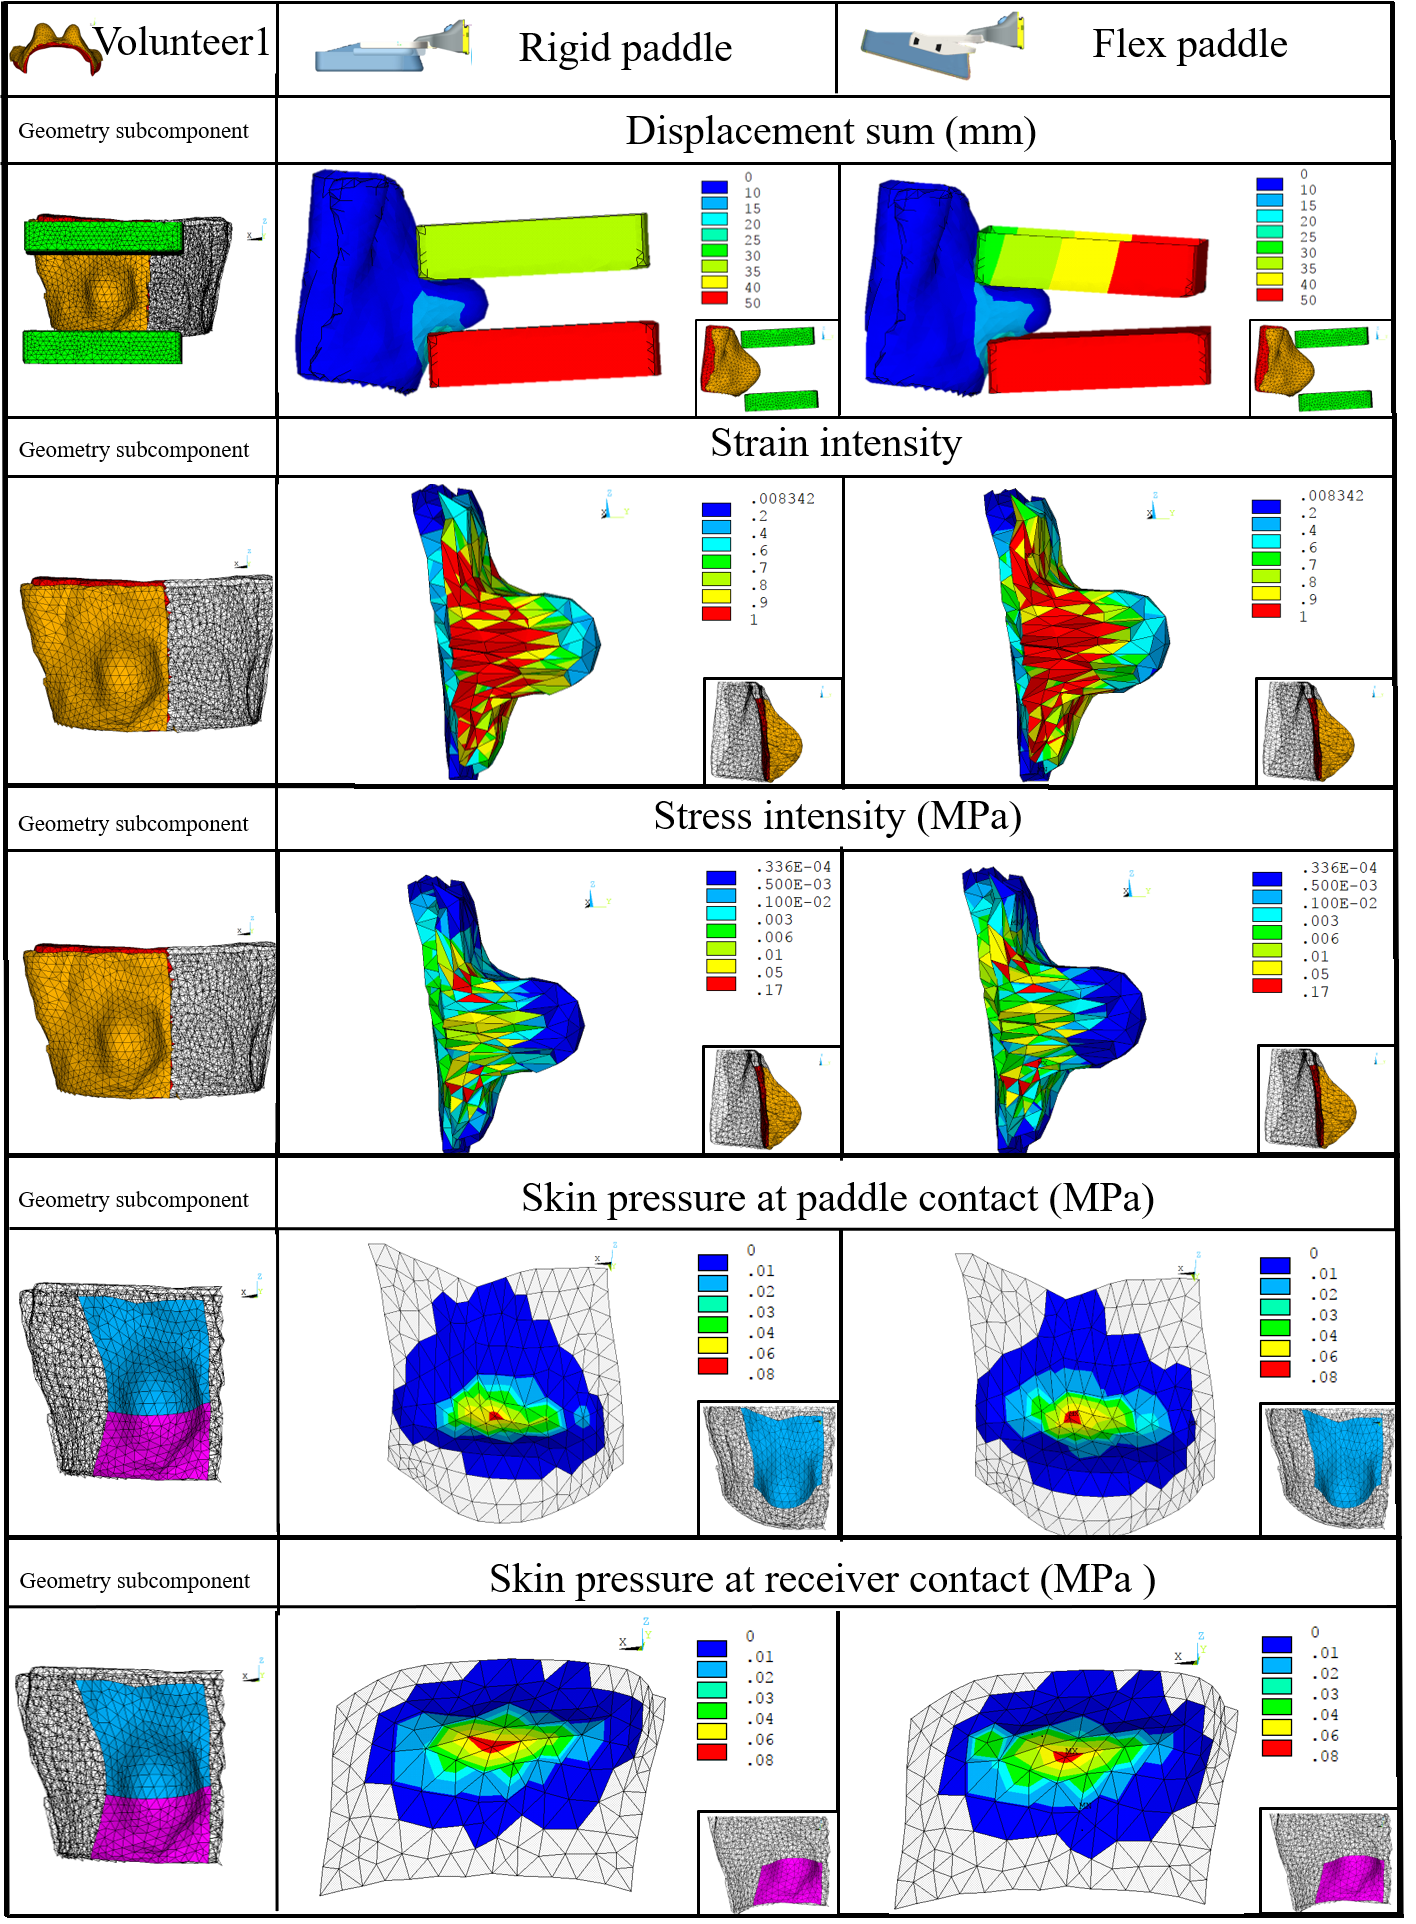
\includegraphics[width=0.95\textwidth,keepaspectratio]{figures/subject1_compressionResults.png} 
\caption{Stress, strain and contact pressure distribution for the first subject}\label{fig:subject1_compressionResults}
\end{figure}

\begin{figure}[!h]
\centering
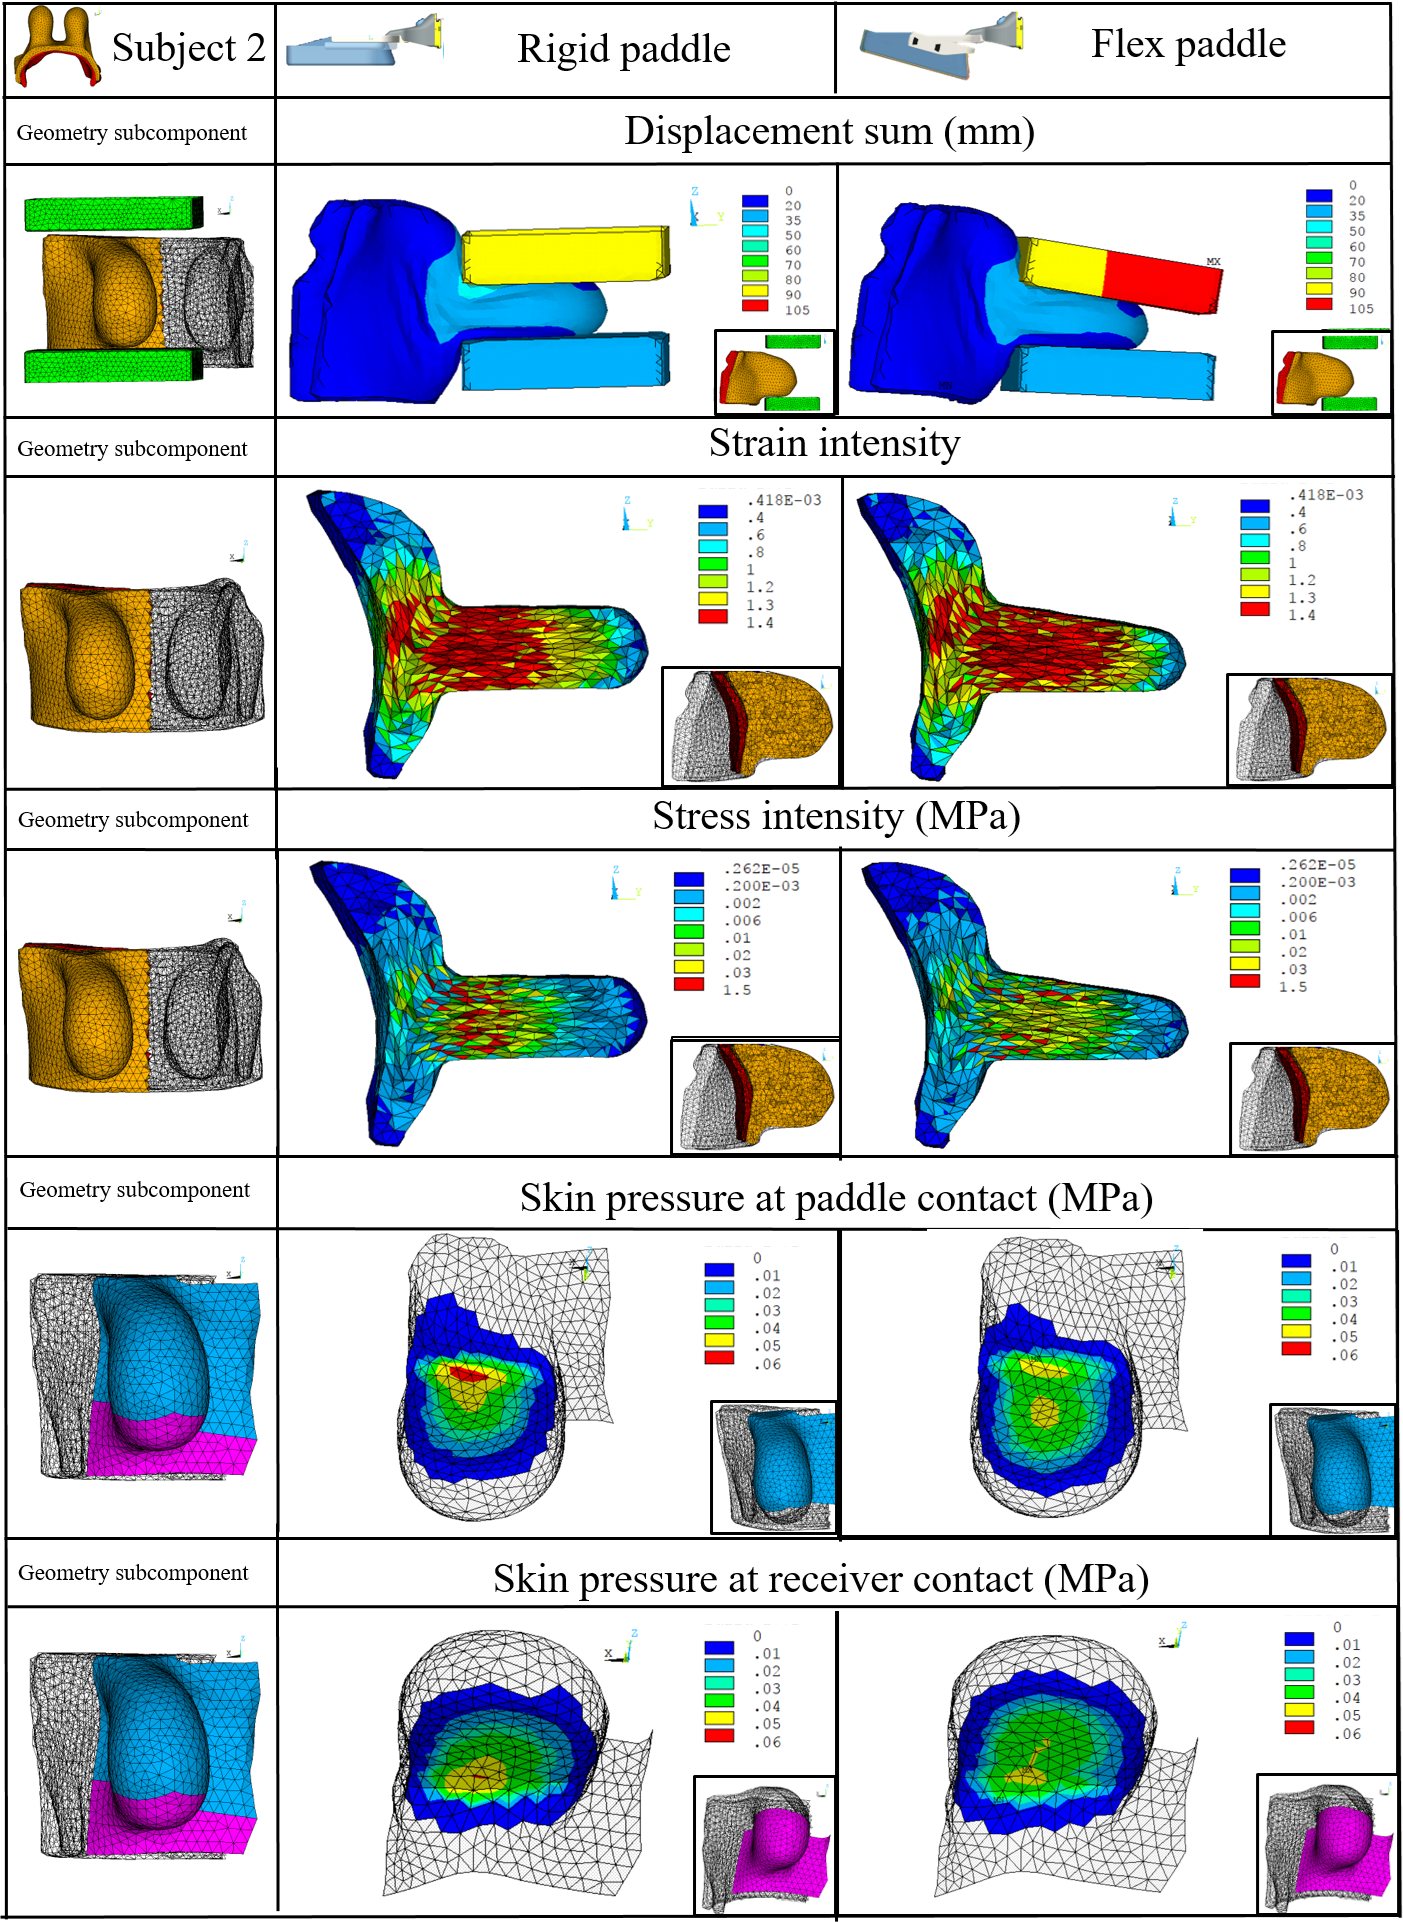
\includegraphics[width=0.95\textwidth,keepaspectratio]{figures/subject2_compressionResults.png} 
\caption{Stress, strain and contact pressure distribution for the second subject}\label{fig:subject2_compressionResults}
\end{figure}

The nominal breast thickness may vary by about 2mm between rigid and flex paddle for both volunteers (Table 3). Accordingly, no significant difference was found between the estimated AGD, while a dose reduction of 2\% for the smaller breast and 4\% for larger breast was observed.

\begin{figure}[!h]
\centering
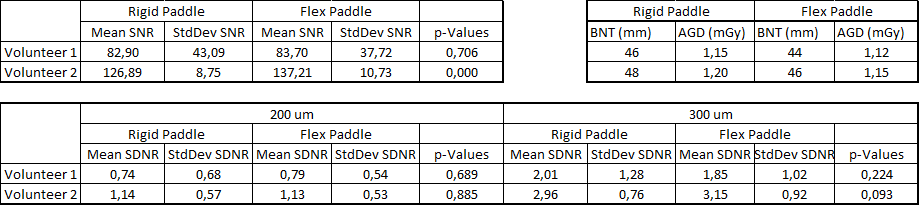
\includegraphics[width=0.95\textwidth,keepaspectratio]{figures/table_compression_results.png} 
\caption{Breast nominal thickness (BNT), average glandular dose (AGD), signal-to-noise-ratio (SNR) and signal-difference-to-noise (SDNR) for both volunteers and both compression paddle types}\label{fig:table_compression_results}
\end{figure}

The SNR and SDNR have been estimated and compared between flex and rigid paddles. When using a flex paddle instead of a rigid paddle on the largest breast (volunteer 2), we observe a statistically significantly higher SNR. The same trend is observed on SDNR for both 200 and 300 µm microcalcifications, while not statistically significant. We did not observe any statistically significant difference in SNR or SDNR for microcalcification of any size when considering the compression of the smallest breast by a rigid or a flex paddle. Therefore, despite a breast thickness varying linearly from chest wall to nipple when the flex compression paddle is used, the image quality is preserved or improves compared to the image quality obtained with the rigid compression paddle.

\section{Discussions and conclusion}\label{section:compressionfem:conclusion}

Breast compression with flex and rigid paddle have been simulated using the finite elements theory applied to segmented MRI images acquired on 2 volunteers under different geometries. Appling the Gent form of strain-energy potential, instead of the Neo-Hookean form, allowed to obtain compression force magnitudes comparable with the real subject data.  
After simulating the breast compression, the SDNR of microcalcifications and the AGD, delivered during the acquisition of the corresponding simulated mammography, have been computed. The simulations have been repeated for two different breast volumes (cup sizes A and F) with a rigid and a flex paddle. The four configurations have been analyzed to compare patient perceived pain (measured as strain and stress) and image quality (measured as SNR, SDNR and AGD). The results of our simulations indicate that, for the smallest breast, there is no significant difference for the patient perceived pain when using the rigid or the flex paddle. The shape of the breast under compression does not present significant changes between the two paddle designs. We did not observe any statistically significant difference in SNR or SDNR for microcalcification of any size when considering the compression of the smallest breast by a rigid or a flex paddle. Therefore, our results suggest that using a flex paddle should not significantly impact image quality and delivered dose in small breasts, and should not reduce significantly the perceived pain.   
For the largest breast, our simulations indicate that using a flex paddle may reduce the maximal pressure intensity on the skin surface by about 30\% compared to the rigid paddle. The tissues deformation is more uniformly distributed inside the breast volume, and the highest deformation is occurring in the middle breast region corresponding to the supposed location of dense tissues. Moreover, our simulations have shown that flex paddle have no significant impact on the average glandular dose and improves image quality compared to the rigid paddle. 
In conclusion, our simulations confirm that using the flex paddle used for breast compression may improve the patient comfort without affecting the image quality and the delivered average glandular dose. Moreover, despite a breast thickness varying linearly from chest wall to nipple, when a flex compression paddle is used on large breasts, the image quality seems to be preserved or improved compared to the image quality obtained with a rigid compression paddle
